%advantages
While magnitude analysis is well-suited for answering research questions about the use of a single IDE command, many research questions are related to a specific feature or tool in the IDE, which usually maps to multiple activities. For instance, the research question ``How often are refactorings performed?'' cannot be answered via magnitude analysis alone, as refactorings can be triggered through a number of different IDE commands. These commands first need to be categorized, after which magnitude analysis can be used. 

%disadvantages
When focusing on a concrete sub-task, such as refactoring, it may be easy to categorize activities. In this case, all refactoring commands, such as pull-up or extract method, can be classified as refactorings. However, when focusing on more general behavior, such as editing, navigating, and searching, categorization can be difficult. It is impossible to say, for instance, from a single click in the {\tt File Explorer} window, whether that click represents a search, as the developers browses a few promising files, or a navigation, as he implicitly opens a type declaration of a variable he was just browsing. Thus, categorization without context can produce noisy data in certain cases. However, categorization is a powerful tool, especially when there is little ambiguity in the IDE commands that are analyzed.

%example
To illustrate both the power and limitations of category analysis consider the following IDE data stream, and the research questions ``Do developers use code search tools?''. 
\begin{figure}
\hrulefill
\begin{verbatim}
Collector Started
2014-02-02 13:21:22 - User submitted query to Find-in-Files
2014-02-02 13:24:36 - Find-in-Files retrieved 42 results
2014-02-02 13:32:21 - User clicked on result 2
2014-02-02 13:46:56 - User submitted query to Quick Find
2014-02-02 14:07:12 - Open definition command; input=class
2014-02-02 14:46:52 - User submitted query to Find-in-Files
2014-02-02 14:46:56 - Find-in-Files retrieved 8 results
2014-02-02 14:48:02 - Click on File Explorer
\end{verbatim}
\hrulefill
	\caption{Log File Search Category Example}
	\label{log:logFileSearch}
\end{figure}


For this research question, the category of log events related to code search tools should be identified and counted. Modern IDEs commonly offer several code search tools, which operate at the global or local scale, such as the {\tt Find-in-Files} and {\tt Quick Find} tools.  An example log from Visual Studio with these tools is shown in Figure \ref{log:logFileSearch} based on Visual Studio. Using categorization analysis we can identify three
log events related to usage of code search tools, and report various statistics aimed at answering the research question (e.g. number of code search events per day, number of code search events per developer see figure \ref{fig:category}). However, the IDE usage data can sometimes be affected by noise, which cannot be avoided by categorization analysis. For instance, the second query to {\tt Find-in-Files} is not followed by a developer click, which is a failed interaction with the {\tt Find-in-Files} tool and should likely not be included in answering the research question.


\begin{figure*}[t]
\centering

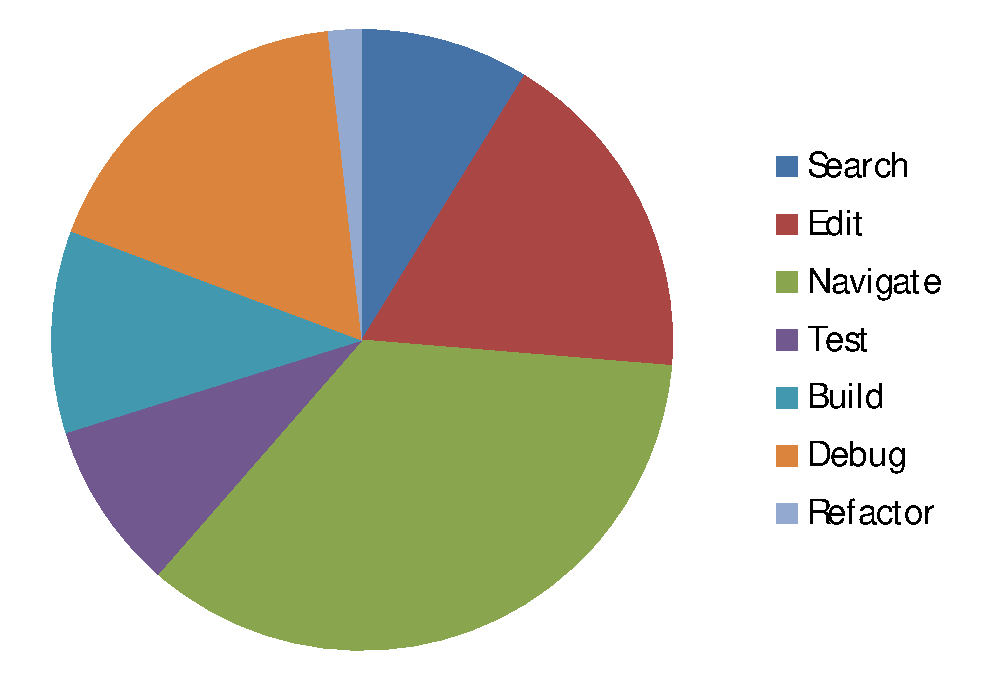
\includegraphics[width=0.5\columnwidth]{activityCategorization.pdf}
\caption{Categorized Log Events with Search Category}
\label{fig:category}
\end{figure*}
